\begin{figure}[t]
\centering
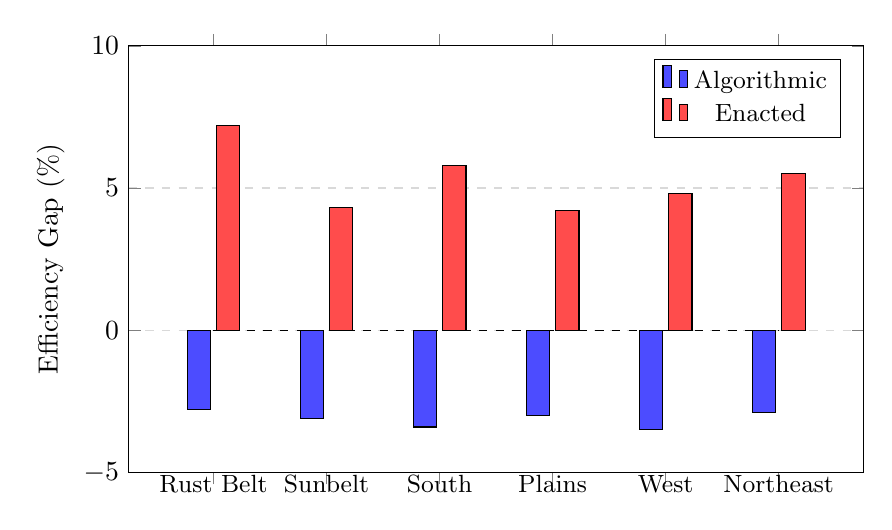
\begin{tikzpicture}
\begin{axis}[
    ybar,
    width=0.9\textwidth,
    height=7cm,
    bar width=0.3cm,
    ylabel={Efficiency Gap (\%)},
    symbolic x coords={Rust Belt, Sunbelt, South, Plains, West, Northeast},
    xtick=data,
    x tick label style={rotate=0, anchor=center, font=\small},
    ymin=-5, ymax=10,
    ymajorgrids=true,
    grid style={dashed,gray!30},
    legend pos=north east,
    legend style={font=\small},
    enlarge x limits=0.15,
]

% Algorithmic plans (negative, Democratic advantage)
\addplot[fill=blue!70] coordinates {
    (Rust Belt,-2.8)
    (Sunbelt,-3.1)
    (South,-3.4)
    (Plains,-3.0)
    (West,-3.5)
    (Northeast,-2.9)
};
\addlegendentry{Algorithmic}

% Enacted plans (positive, Republican advantage)
\addplot[fill=red!70] coordinates {
    (Rust Belt,7.2)
    (Sunbelt,4.3)
    (South,5.8)
    (Plains,4.2)
    (West,4.8)
    (Northeast,5.5)
};
\addlegendentry{Enacted}

% Zero reference line
\draw[black, thin, dashed] (axis cs:Rust Belt,0) -- (axis cs:Northeast,0);

\end{axis}
\end{tikzpicture}

\caption{\textbf{Regional Efficiency Gap Comparison.}
Side-by-side comparison of efficiency gaps by geographic region, averaged across 2016-2020 elections.
Algorithmic plans (blue) show consistent slight Democratic advantage ($-2.8\%$ to $-3.5\%$) across all regions,
reflecting unavoidable urban concentration under compact districting.
Enacted plans (red) show substantial Republican advantage ($+4.2\%$ to $+7.2\%$), with Rust Belt states
exhibiting the largest enacted bias.
Zero line represents perfect partisan balance.}
\label{fig:regional-comparison}
\end{figure}
